\documentclass[]{article}
\usepackage[utf8]{inputenc}

\usepackage{anyfontsize}

\usepackage{float}

\usepackage{geometry}
\geometry{
	right=35mm,
	left=35mm,
	top=30mm,
	bottom=30mm
}

%\usepackage{fontspec}
%\setmainfont{Arial}

\usepackage{titlesec}

\usepackage{setspace}
\setstretch{1.2}

\usepackage[linesnumbered, ruled, lined, boxed]{algorithm2e}

\titlespacing*{\section}{0cm}{1cm}{1cm}

\setlength{\interspacetitleruled}{5pt}

\title{\raggedright \bf \fontsize{32}{32}\selectfont{Algoritmos}}
\author{}
\date{}

\SetKwInput{KwData}{Datos de entrada}
\SetKwInput{KwResult}{Resultado}

\IncMargin{1em}

\newlength{\grosor}
\setlength{\grosor}{1pt}

\makeatletter
\let\old@algocf@pre@ruled\@algocf@pre@ruled
\renewcommand{\@algocf@pre@ruled}{\hrule width\algocf@ruledwidth height\grosor depth0pt\kern\interspacetitleruled}
\makeatother

\newlength{\espacioVert}
\setlength{\espacioVert}{0.5cm}

\let\oldnl\nl
\newcommand{\nonl}{\renewcommand{\nl}{\let\nl\oldnl}}

\usepackage[table]{xcolor}

\usepackage{tikz}



\begin{document}



\maketitle

\section*{Algoritmo 1}

%{\bf Información}: Determinar qué símbolos usar si la base es mayor a $10$. \\

\SetAlgorithmName{Algoritmo}{}{}

\DontPrintSemicolon


\begin{algorithm}[H]
	
	\vspace{\espacioVert}

	\KwData{Num. renglones $n$; num. columnas $m$; cantidades de objetos por clase $N_1$, $N_2$; mallas $2\times2$ óptimas.}
	\KwResult{Malla con objetos acomodados (representada por una matriz de enteros).}
	
	\vspace{\espacioVert}	
	
	Declaraciones y casos especiales (ver descripción \ref{algo2}).
	
	\vspace{\espacioVert}	
	
	\tcp*[l]{Correr ventana en la malla. Los indices $i$ y $j$ recorren las celdas de la malla y corresponden a la esquina inferior
	derecha de la ventana.}
	
	\For{$i=2,\ i\leq n,\ i++$}{
	
		\For{$j=2,\ j\leq m,\ j++$}{
		
			\vspace{\espacioVert}	
		
			Decidir qué elementos colocar en ventana (ver descripción \ref{algo3}).
			
			\vspace{\espacioVert}	
			
			Hacer que los elementos de la ventana coincidan con los elementos ya colocados en la malla y colocarlos (ver descripción 
			\ref{algo4}).
			
			\vspace{\espacioVert}	
		}
	}
	
	\vspace{\espacioVert}	
	
	Arreglar cuadros imposibles (ver descripción \ref{algo5}).
	
	\vspace{\espacioVert}	
	
	\caption{Recorrido ventana. Complejidad: $O(x)$.}

\end{algorithm}


\SetAlgorithmName{Descripción}{}{}
\setcounter{algocf}{0}


\begin{algorithm}[H]
	
	\vspace{\espacioVert}		
	
	Declarar de mallas $2\times2$ óptimas.
	
	$int\ N = N_1 + N_2$ \tcp*[r]{Total de objetos.}
	
	\vspace{\espacioVert}	
	
	\tcp*[l]{Verificar si es caso trivial.}
	\If{$N < ceil\left({|n\times m| \over 2}\right)$}{Caso trivial, resolver con el patrón establecido.}
	
	\vspace{\espacioVert}
	
	\tcp*[l]{Condición para que haya al menos 1 caso imposible.}
	\If{$max(\{N_1,N_2\})>(|n\times m| - floor(n/2)*floor(m/2))$}{Hay casos imposibles en el arreglo.}
	
	\vspace{\espacioVert}
	
	Inicializar malla con todos sus valores iguales a $-1$, ya que si fueran $0$'s habría problemas a la hora de hacer calculos 
	relacionados con el número de vacíos.
	
	\vspace{\espacioVert}	

	\caption{Declaraciones y casos especiales.\label{algo2}}

\end{algorithm}


%\vspace{1cm}


\begin{algorithm}[H]

	\vspace{\espacioVert}	
			
			\tcp*[l]{Declarar vector que contiene el número de objetos de cada clase que contendrá la ventana. Así como la variable que 				contiene el número de espacios a llenar de la ventana.}
			$int\ v\_elem = \{0,0\}$\;
			$int\ espacios\_a\_llenar$\;
			
			\vspace{\espacioVert}	
			
			Contar el número de espacios a llenar de la ventana (contar los $-1$'s) y poner el valor en $espacios\_a\_llenar$.\;
			
			\vspace{\espacioVert}	
			
			Contar cuántos objetos de cada clase ya hay en la ventana y ponerlos en $v\_elem$.\;
			
			\vspace{\espacioVert}	
			
			\While{$espacios\_a\_llenar>0$}{
			
				\vspace{\espacioVert}	
				
				\tcp*[l]{Elegir los objetos a colocar en la ventana con el criterio basado en mayorias (tomar primero de los que hay 
				más).}
				Determinar de qué clase hay más objetos para colocar.\;

				\vspace{\espacioVert}	
				
				Poner el objeto de tal clase en la ventana, es decir, hacer las actualizaciones correspondientes a $v\_elem$, $espacios
				\_a\_llenar$, etc.\;
				
				\vspace{\espacioVert}	
			}
			
			\vspace{\espacioVert}	

	\caption{Decidir qué elementos colocar en ventana. \label{algo3}}

\end{algorithm}


\vspace{1cm}


\begin{algorithm}[H]

	\tcp*[l]{El vector $v\_elem$ es la clave de un diccionario, al cual se le da el número de elementos de cada clase que tiene 				la ventana y te regresa una de las matrices de $2\times 2$ óptimas con ese número de elementos.}
			$matrizOptima = dic\_matOptimas(v\_elem)$\;
			
	\vspace{\espacioVert}	
	\tcp*[l]{Inician casos para ver en qué zona de la malla se encuentra la ventana (las zonas están en la imagen del Word).}
	\Case{$i==2 \wedge j==2$}{
		Colocar los 4 elementos de $matrizOptima$ en la malla.
	}
	
	\Case{$i==2 \wedge j>2$}{
		Rotar y reflejar la $matrizOptima$, hasta que los 2 elementos de su izquierda coincidan con los elementos ya colocados 
		en la malla (aquí es mucho código, ya que hay que hacer operaciones para cada caso de rotación y reflexión).\;
		\vspace{\espacioVert}	
		Colocar los elementos de $matrizOptima$ en la malla.
	}
			
	\vspace{\espacioVert}	
			
	\Case{$i>2 \wedge j==2$}{
		Rotar y reflejar la $matrizOptima$, hasta que sus 2 elementos superiores coincidan con los elementos ya colocados en la 					malla (aquí es mucho código, ya que hay que hacer operaciones para cada caso de rotación y reflexión).\;
		\vspace{\espacioVert}	
		Colocar los elementos de $matrizOptima$ en la malla.
	}
			
	\vspace{\espacioVert}	
			
	\Case{$i>2 \wedge j>2$}{
		Rotar y reflejar la $matrizOptima$, hasta que coincida con los 3 elementos ya colocados en la malla (aquí es mucho 						código, ya que hay que hacer operaciones para cada caso de rotación y reflexión).\;
		\vspace{\espacioVert}	
		Colocar los elementos de $matrizOptima$ en la malla.
	}
	
	\tcp*[l]{Ver comantarios pag. 5.}

	\caption{Hacer que elementos de ventana coincidan con los ya colocados y colocarlos. \label{algo4}}

\end{algorithm}


\setlength{\algoheightrule}{0pt}
\setlength{\grosor}{0pt}
\setlength{\algotitleheightrule}{0pt}
\setlength{\interspacetitleboxruled}{0pt}

\SetKwFor{For}{}{}{end}


\begin{algorithm}[H]
	
	\tcp*[l]{Una vez colocados todos los objetos en la malla, se verifica si hay casos imposibles, para esto se recorren los puntos clave 	de la malla (los que están en verde en el Word). Cada celda, y por lo tanto cada punto clave puede ser parte de 1 a 4 cuadros
	imposibles de $2\times 2$. Si los ocho objetos que rodean al punto clave son iguales a este, se da el peor de los casos (4 cuadros
	imposibles).}
	\vspace{\espacioVert}	
	\tcp*[l]{Basta con que el elemento del punto clave sea diferente de los objetos que lo rodean para que no haya ningún cuadro
	imposible en esas 9 celdas. Por lo que el proceso para arreglar los casos imposibles consiste en intercambiar el elemento del punto
	clave que pertenece a un cuadro imposible, con uno de su vecindad que sea diferente, o con uno de la vecindad de otro punto clave (en
	este caso, la vecindad de un punto clave son los 8 elementos que lo rodean).}
	
\end{algorithm}


\setlength{\algoheightrule}{1pt}
\setlength{\grosor}{1pt}
\setlength{\algotitleheightrule}{1pt}
\setlength{\interspacetitleboxruled}{1pt}

\SetKwFor{For}{for}{do}{end}


\begin{algorithm}[H]

	\vspace{\espacioVert}	

	\tcp*[l]{Se declara una matriz de casos imposibles. El número de elementos de esta matriz es el número de puntos claves en la malla (como si se construyera una matriz solo con los puntos verdes). Cada elemento de la matriz indica el número de casos imposibles de los que es parte un punto clave (de 0 a 4).}
	$int\ matrizImposibles[][]$\;
	
	\vspace{\espacioVert}	
	
	Se recorre la ventana para contar los casos imposibles de cada punto clave y registrarlos en $matrizImposibles$\;
	
	\vspace{\espacioVert}	

	\tcp*[l]{Correr indices en matriz de casos imposibles.}

	\For{$i=1,\ i\leq renglonesMatrizImposibles,\ i++$}{
	
		\For{$j=1,\ j\leq columnasMatrizImposibles,\ j++$}{
		
		\vspace{\espacioVert}	
		
			\If(\tcp*[r]{Si hay un casos imposibles.}){$matrizImposibles[i][j]>0$}{

				Verificar vecinos del punto clave correspondiente en busca de un elemento diferente.\;
				
				\vspace{\espacioVert}	
				
				\If{Todos los vecinos son iguales al punto clave.}{
				
					Buscar en vecindades de los demás puntos claves.
				}
				
				\vspace{\espacioVert}	
				
				Intercambiar elemento de punto clave con el elemento encontrado.\;
				
				\vspace{\espacioVert}	
				
				Actualizar matriz de casos imposibles.
			}
		}
	}
	
	%\vspace{\espacioVert}	
	
	\tcp*[l]{Es en las líneas de la 9 a la 12 donde también se lleva gran cantidad de código, ya que para recorrer los 8 vecinos
	de cada punto clave se requieren varios $if$'s. Si bien al hacer el intercambio se liberan los cuadros imposibles de un lado, hay que 
	verificar que del otro no se generen más, y de ser así hay que actualizar la matriz de casos imposibles, o sea, hay que ver a qué
	punto clave pertenece los imposibles generados al hacer el intercambio.}
	\vspace{\espacioVert}	
	\tcp*[l]{Y para todo lo anterior hay que estar verificando en qué 
	zona de la malla se está, porque no es lo mismo una vecindad de la parte central de la malla que en un borde o una esquina (se 
	dice fácil pero se lleva mucho código).}
	
	\caption{Arreglar cuadros imposibles. \label{algo5}}

\end{algorithm}


\section*{Algoritmo 2}

%{\bf Información}: Determinar qué símbolos usar si la base es mayor a $10$. \\

\SetAlgorithmName{Algoritmo}{}{}
\setcounter{algocf}{1}

\begin{algorithm}[H]

	\vspace{\espacioVert}

	\KwData{Num. renglones $n$; num. columnas $m$; cantidades de objetos por clase $N_1$, $N_2$; diccionarios vecindades$\rightarrow$puntajes.}
	\KwResult{Malla con objetos acomodados (representada por una matriz de enteros).}
	
	\vspace{\espacioVert}
	
	Declaraciones (ver descripción \ref{algo7}).
	
	\vspace{\espacioVert}
	
	Función $puntajeElemento()$ (ver función \ref{algo8}).
	
	\vspace{\espacioVert}
	
	Función $puntajeCruzElemento()$ (ver función \ref{algo9}).
	
	\vspace{\espacioVert}
	
	\tcp*[l]{Finalizan declaraciones y comienza la ejecución del programa.}
	
	\vspace{\espacioVert}
	
	Casos triviales e inicializaciones (ver descripción \ref{algo10}).
	
	\vspace{\espacioVert}
	
	\tcp*[l]{Bucle para mejorar el puntaje de la malla. Uso este formato de indices para no poner 4 $for$'s.}
	
	\For{$indice1$ {\bf in} $matricesPuntajes[1]$}{
	
		\For{$indice2$ {\bf in} $matricesPuntajes[1]$}{

			\tcp*[l]{Si los elementos son iguales, no hacer nada.}
			\If{$malla[indice1] == malla[indice2]$}{Saltar a la sig. iteración.}
			
			\vspace{\espacioVert}
			
			Comparar puntajes y hacer cambio si conviene (ver descripción \ref{algo11}).
		}
	}
	
	\vspace{\espacioVert}
	
	\caption{Aprendizaje por refuerzo. Complejidad: $O(3x + 24*\#intercambios)$?.}

\end{algorithm}


\SetAlgorithmName{Descripción}{}{}
\setcounter{algocf}{4}


\begin{algorithm}[H]

	\vspace{\espacioVert}
	
	$int\ N = N_1 + N_2$ \tcp*[r]{Total de objetos.}
	
	\vspace{\espacioVert}
	
	\tcp*[l]{Declarar contador para llevar registro de las iteraciones seguidas en las que no mejoró la puntuación de la malla.}
	$int\ contSinCambios$\;
	
	\vspace{\espacioVert}	
	
	\tcp*[l]{Declarar diccionarios con la información vecindades$\rightarrow$puntajes para cada zona de la malla (uno para esquinas, uno para bordes y uno para el centro). Un ejemplo de los puntajes está en la imágen de Word.}
	$dicVecindadesPuntajesEsq$\;
	$dicVecindadesPuntajesBordes$\;
	$dicVecindadesPuntajesCentro$\;
	
	\vspace{\espacioVert}
	
	\tcp*[l]{Declarar matriz donde se guarda el puntaje de cada elemento, dado por los diccionarios.}
	$matPunt[n][m]$\;
	
	\vspace{\espacioVert}

	\tcp*[l]{La explicación de las siguientes matrices es la parte más difícil de entender. Si no le entiende, tómelo solo como una 
	matriz que contiene las puntuaciones de los elementos de la malla (similar a la anterior) y siga con lo demás.}
	
	\vspace{\espacioVert}
	
	\tcp*[l]{Declarar matrices de puntajes en cruz. Este es un arreglo de $3\times n \times m$ (el 3 es por la cantidad de elementos 
	diferentes que se pueden colocar en la malla: 1's, 2,s y 0's) donde, en cada celda de la primera matriz se guarda la suma de los 
	siguientes puntajes de $matPunt[n][m]$: el del elemento en cuestión + el de sus 4 vecinos. Estos son los puntajes del estado actual 
	de la malla, las otras 2 matrices se calculan haciendo lo mismo pero cambiando el elemento en cuestión o central por los otros 2 
	elementos (si hay un 1 en el estado actual, ahora se supondrá que hay un 2 para una matriz y un cero para la otra, los vecinos no 
	cambian).}
	$matricesPuntajes[3][n][m]$\;
	
	\vspace{\espacioVert}

	\caption{Declaraciones. \label{algo7}}

\end{algorithm}


\SetKwProg{Fn}{function}{:}{end}
\SetAlgorithmName{Función}{}{}
\setcounter{algocf}{0}


\begin{algorithm}[H]

	\vspace{\espacioVert}
	
	\tcp*[l]{Función para calcular puntaje de un elemento de $matPunt[n][m]$. Verifica en qué parte de la malla se encuentra el elemento 
	y llama al 
	diccionario adecuado.}
	\Fn{puntajeElemento(int renglon, int columna)}{
	
		\vspace{\espacioVert}
	
		$int\ vectorVecindad[4]$
		
		\vspace{\espacioVert}
		
		Obtener la vecindad del elemento y ponerla en $vectorVecindad$.
		
		\vspace{\espacioVert}
		
		\Case{Elemento en esquinas}{
		
			return $dicVecindadesPuntajesEsq(vectorVecindad)$
		}
		
		\vspace{\espacioVert}
		
		\Case{Elemento en bordes}{
		
			return $dicVecindadesPuntajesBordes(vectorVecindad)$
		}
		
		\vspace{\espacioVert}
		
		\Case{Elemento en centro}{
		
			return $dicVecindadesPuntajesCentro(vectorVecindad)$
		}
	}
	
	\vspace{\espacioVert}

	\caption{Función $puntajeElemento()$. \label{algo8}.}

\end{algorithm}


\begin{algorithm}[H]
	
	\vspace{\espacioVert}
	
	\tcp*[l]{Función para calcular puntaje de un elemento de $matricesPuntajes$.}
	\Fn{puntajeCruzElemento(int renglon, int columna)}{
	
		\vspace{\espacioVert}
		
		\tcp*[l]{Caso para los puntajes actuales. Para los otros 2 puntajes supuestos el código es similar. Son supuestos por que se 
		supone que el elemento se cambia por otro distinto.}
		$puntaje = matPunt[renglon][columna]$\;
		\lIf{$renglon>1$}{$puntaje += matPunt[renglon-1][columna]$}
		\lIf{$renglon<n$}{$puntaje += matPunt[renglon+1][columna]$}
		\lIf{$columna>1$}{$puntaje += matPunt[renglon][columna-1]$}
		\lIf{$columna<m$}{$puntaje += matPunt[renglon][columna+1]$}
		
		\vspace{\espacioVert}
		
		return $puntaje$
	}
	
	\vspace{\espacioVert}
	
	\caption{Función $puntajeCruzElemento()$. \label{algo9}.}

\end{algorithm}


\SetAlgorithmName{Descripción}{}{}
\setcounter{algocf}{5}


\begin{algorithm}[H]

	\vspace{\espacioVert}
	
	\tcp*[l]{Verificar si es caso trivial.}
	\If{$N < ceil\left({|n\times m| \over 2}\right)$}{Caso trivial, resolver con el patrón establecido.}
	
	\vspace{\espacioVert}

	\tcp*[l]{Condición para que haya al menos 1 caso imposible.}
	\If{$max(\{N_1,N_2\})>(|n\times m| - floor(n/2)*floor(m/2))$}{Hay casos imposibles en el arreglo.}
	
	\vspace{\espacioVert}
	
	Inicializar la malla aleatoriamente con la cantidad $N_1$ de cubos (1's) y $N_2$ de prismas (2's, los vacíos aquí si son 0's).\;
	
	\vspace{\espacioVert}
	
	Llenar los puntajes de $matPunt[n][m]$ mediante la función $puntajeElemento()$.\;
	
	\vspace{\espacioVert}
	
	A partir de los puntajes anteriores llenar la información de $matricesPuntajes[1][n][m]$ y calcular lo puntajes para las otras 2 
	matrices, mediante la función $puntajeCruzElemento()$.\;
	
	\vspace{\espacioVert}
	
	\tcp*[l]{Hasta aquí llevamos los $3x$ de complejidad (se supone que cada vez que se llena una de las 3 matrices es una $x$).}
	
	\vspace{\espacioVert}

	\caption{Casos triviales e inicializaciones. \label{algo10}}

\end{algorithm}


\begin{algorithm}[H]
			
	\vspace{\espacioVert}
		
	$puntajeActual = matricesPuntajes[1][indice1] + matricesPuntajes[1][indice2]$\;
	\tcp*[l]{El puntaje ya calculado del intercambio está en las matrices de puntajes supuestos, ya sea la 2 o la 3.}
	$puntajeIntercambio = matricesPuntajes[2][indice1] + matricesPuntajes[3][indice2]$ 

	\vspace{\espacioVert}

	\eIf{$puntajeIntercambio > puntajeActual$}{
			
		\vspace{\espacioVert}
			
		$contSinCambios=0$\;
			
		\vspace{\espacioVert}
			
		Hacer el intercambio de elementos. Esto es: intercambiar los elementos en la $malla$, cambiar los puntajes actuales por los de 
		intercambio en $matricesPuntajes$ y actualizar $matPunt$ de los 2 elementos en cuestión.\;
				
		\vspace{\espacioVert}
				
		Actualizar los puntajes de los vecinos de los elementos intercambiados en $matricesPuntajes$ y en $matPunt$ (los puntajes de los 
		elementos intercambiados ya están actualizados con la línea anterior).\;
			
		\vspace{\espacioVert}
				
		\tcp*[l]{Es en la línea anterior donde aparece el segundo término de complejidad: $24*\#intercambios$. Ya que en totalson 8 
		vecinos y hay que actualizar sus 3 puntajes en $matricesPuntajes$ (el actual y los supuestos), de ahí el 24 (8*3).}
				
	}{
			
		$contSinCambios++$\;
	}
			
	\vspace{\espacioVert}
			
	\SetKwIF{If}{ElseIf}{Else}{if}{then}{else if}{else}{end}
			
	\lIf(\tcp*[l]{Condición de paro}){$contSinCambios>ciertoLimite$}{Terminar.}
			
	\tcp*[l]{Es en las líneas de la 1 a la 3 donde sí se realizan esas operaciones con complejidad cuadrática. Pero si las ve, solo son 2 
	sumas y 2 comparaciones, que comparadas con las operaciones a las que sí tomo en cuenta para la complejidad, son muy pocas, por lo 
	que no las tomo en cuenta, ¿estoy bien en no tomarlas en cuenta?. Esa es la duda por la que no sé si ponerle complejidad lineal + el 
	otro término al algoritmo o no.}
			
	\vspace{\espacioVert}
				
	\caption{Comparar puntajes y hacer cambio si conviene. \label{algo11}.}


\end{algorithm}


\pagebreak


\section*{Algunos ejemplos}


\renewcommand{\arraystretch}{2.5}

Se muestran ejemplos del acomodo de los 2 algoritmos y la suma de movimientos para acceder a todos los objetos.

\vspace{1cm}

{\Large \bf \hspace{0.0cm} Acomodo Refuerzo \hspace{3cm} Acomodo Ventana}

\vspace{1cm}

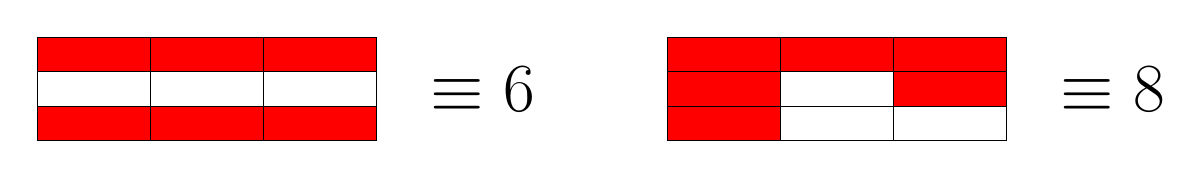
\begin{tikzpicture}
  \node at (-2,0) {
  \begin{tabular}{|m{1cm}|m{1cm}|m{1cm}|}
	\hline
	\cellcolor{red} & \cellcolor{red} & \cellcolor{red} \tabularnewline \hline
	 &  &  \tabularnewline \hline
	\cellcolor{red} & \cellcolor{red} & \cellcolor{red} \tabularnewline \hline
  \end{tabular}
  };
  \node at (1.5,0) {\Huge $\equiv 6$};
  
  \node at (6,0) {
  \begin{tabular}{|m{1cm}|m{1cm}|m{1cm}|}
	\hline
	\cellcolor{red} & \cellcolor{red} & \cellcolor{red} \tabularnewline \hline
	\cellcolor{red} & \cellcolor{white} & \cellcolor{red} \tabularnewline \hline
	\cellcolor{red} & \cellcolor{white} & \cellcolor{white} \tabularnewline \hline
  \end{tabular}
  };
  \node at (9.5,0) {\Huge $\equiv 8$};
\end{tikzpicture}

\vspace{1cm}

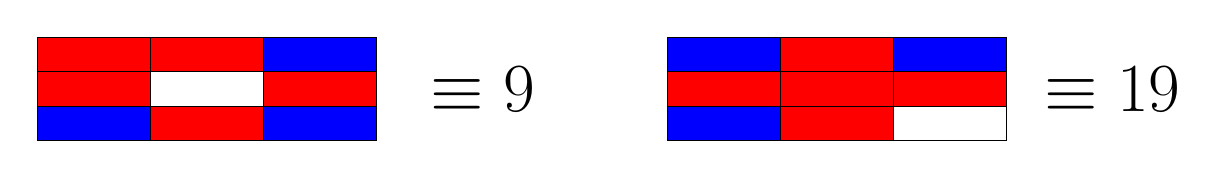
\begin{tikzpicture}
  \node at (-2,0) {
  \begin{tabular}{|m{1cm}|m{1cm}|m{1cm}|}
	\hline
	\cellcolor{red} & \cellcolor{red} & \cellcolor{blue} \tabularnewline \hline
	\cellcolor{red} & \cellcolor{white} & \cellcolor{red} \tabularnewline \hline
	\cellcolor{blue} & \cellcolor{red} & \cellcolor{blue} \tabularnewline \hline
  \end{tabular}
  };
  \node at (1.5,0) {\Huge $\equiv 9$};
  
  \node at (6,0) {
  \begin{tabular}{|m{1cm}|m{1cm}|m{1cm}|}
	\hline
	\cellcolor{blue} & \cellcolor{red} & \cellcolor{blue} \tabularnewline \hline
	\cellcolor{red} & \cellcolor{red} & \cellcolor{red} \tabularnewline \hline
	\cellcolor{blue} & \cellcolor{red} & \cellcolor{white} \tabularnewline \hline
  \end{tabular}
  };
  \node at (9.5,0) {\Huge $\equiv 19$};
\end{tikzpicture}

\vspace{1cm}

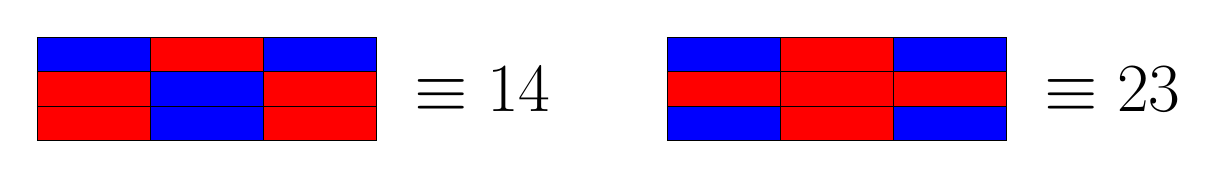
\begin{tikzpicture}
  \node at (-2,0) {
  \begin{tabular}{|m{1cm}|m{1cm}|m{1cm}|}
	\hline
	\cellcolor{blue} & \cellcolor{red} & \cellcolor{blue} \tabularnewline \hline
	\cellcolor{red} & \cellcolor{blue} & \cellcolor{red} \tabularnewline \hline
	\cellcolor{red} & \cellcolor{blue} & \cellcolor{red} \tabularnewline \hline
  \end{tabular}
  };
  \node at (1.5,0) {\Huge $\equiv 14$};
  
  \node at (6,0) {
  \begin{tabular}{|m{1cm}|m{1cm}|m{1cm}|}
	\hline
	\cellcolor{blue} & \cellcolor{red} & \cellcolor{blue} \tabularnewline \hline
	\cellcolor{red} & \cellcolor{red} & \cellcolor{red} \tabularnewline \hline
	\cellcolor{blue} & \cellcolor{red} & \cellcolor{blue} \tabularnewline \hline
  \end{tabular}
  };
  \node at (9.5,0) {\Huge $\equiv 23$};
\end{tikzpicture}


\pagebreak


\renewcommand{\arraystretch}{2.05}


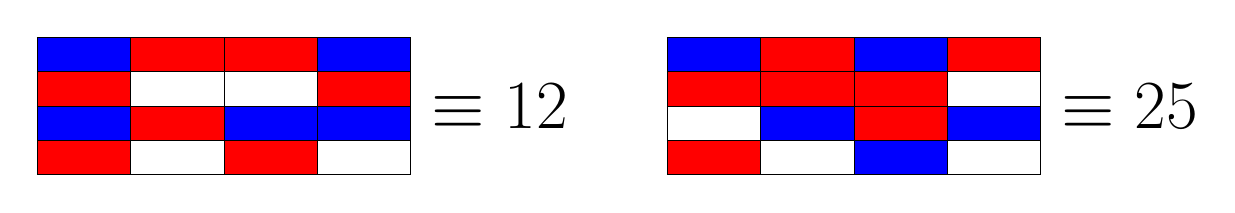
\begin{tikzpicture}
  \node at (-2,0) {
  \begin{tabular}{|m{0.75cm}|m{0.75cm}|m{0.75cm}|m{0.75cm}|}
	\hline
	\cellcolor{blue} & \cellcolor{red} & \cellcolor{red} & \cellcolor{blue} \tabularnewline \hline
	\cellcolor{red} & \cellcolor{white} & \cellcolor{white} & \cellcolor{red} \tabularnewline \hline
	\cellcolor{blue} & \cellcolor{red} & \cellcolor{blue} & \cellcolor{blue} \tabularnewline \hline
	\cellcolor{red} & \cellcolor{white} & \cellcolor{red} & \cellcolor{white} \tabularnewline \hline
  \end{tabular}
  };
  \node at (1.5,0) {\Huge $\equiv 12$};
  
  \node at (6,0) {
  \begin{tabular}{|m{0.75cm}|m{0.75cm}|m{0.75cm}|m{0.75cm}|}
	\hline
	\cellcolor{blue} & \cellcolor{red} & \cellcolor{blue} & \cellcolor{red} \tabularnewline \hline
	\cellcolor{red} & \cellcolor{red} & \cellcolor{red} & \cellcolor{white} \tabularnewline \hline
	\cellcolor{white} & \cellcolor{blue} & \cellcolor{red} & \cellcolor{blue} \tabularnewline \hline
	\cellcolor{red} & \cellcolor{white} & \cellcolor{blue} & \cellcolor{white} \tabularnewline \hline
  \end{tabular}
  };
  \node at (9.5,0) {\Huge $\equiv 25$};
\end{tikzpicture}

\vspace{2cm}

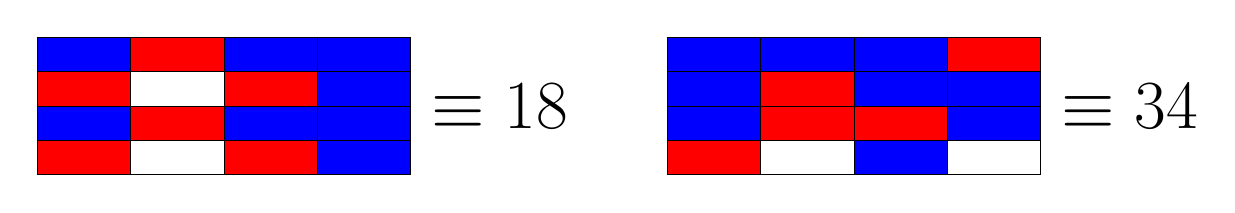
\begin{tikzpicture}
  \node at (-2,0) {
  \begin{tabular}{|m{0.75cm}|m{0.75cm}|m{0.75cm}|m{0.75cm}|}
	\hline
	\cellcolor{blue} & \cellcolor{red} & \cellcolor{blue} & \cellcolor{blue} \tabularnewline \hline
	\cellcolor{red} & \cellcolor{white} & \cellcolor{red} & \cellcolor{blue} \tabularnewline \hline
	\cellcolor{blue} & \cellcolor{red} & \cellcolor{blue} & \cellcolor{blue} \tabularnewline \hline
	\cellcolor{red} & \cellcolor{white} & \cellcolor{red} & \cellcolor{blue} \tabularnewline \hline
  \end{tabular}
  };
  \node at (1.5,0) {\Huge $\equiv 18$};
  
  \node at (6,0) {
  \begin{tabular}{|m{0.75cm}|m{0.75cm}|m{0.75cm}|m{0.75cm}|}
	\hline
	\cellcolor{blue} & \cellcolor{blue} & \cellcolor{blue} & \cellcolor{red} \tabularnewline \hline
	\cellcolor{blue} & \cellcolor{red} & \cellcolor{blue} & \cellcolor{blue} \tabularnewline \hline
	\cellcolor{blue} & \cellcolor{red} & \cellcolor{red} & \cellcolor{blue} \tabularnewline \hline
	\cellcolor{red} & \cellcolor{white} & \cellcolor{blue} & \cellcolor{white} \tabularnewline \hline
  \end{tabular}
  };
  \node at (9.5,0) {\Huge $\equiv 34$};
\end{tikzpicture}

\vspace{2cm}

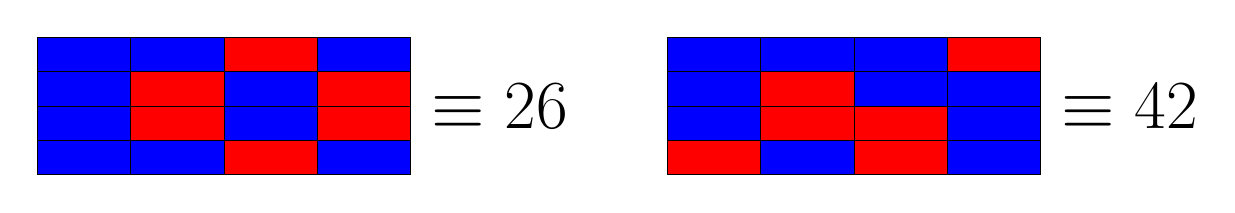
\begin{tikzpicture}
  \node at (-2,0) {
  \begin{tabular}{|m{0.75cm}|m{0.75cm}|m{0.75cm}|m{0.75cm}|}
	\hline
	\cellcolor{blue} & \cellcolor{blue} & \cellcolor{red} & \cellcolor{blue} \tabularnewline \hline
	\cellcolor{blue} & \cellcolor{red} & \cellcolor{blue} & \cellcolor{red} \tabularnewline \hline
	\cellcolor{blue} & \cellcolor{red} & \cellcolor{blue} & \cellcolor{red} \tabularnewline \hline
	\cellcolor{blue} & \cellcolor{blue} & \cellcolor{red} & \cellcolor{blue} \tabularnewline \hline
  \end{tabular}
  };
  \node at (1.5,0) {\Huge $\equiv 26$};
  
  \node at (6,0) {
  \begin{tabular}{|m{0.75cm}|m{0.75cm}|m{0.75cm}|m{0.75cm}|}
	\hline
	\cellcolor{blue} & \cellcolor{blue} & \cellcolor{blue} & \cellcolor{red} \tabularnewline \hline
	\cellcolor{blue} & \cellcolor{red} & \cellcolor{blue} & \cellcolor{blue} \tabularnewline \hline
	\cellcolor{blue} & \cellcolor{red} & \cellcolor{red} & \cellcolor{blue} \tabularnewline \hline
	\cellcolor{red} & \cellcolor{blue} & \cellcolor{red} & \cellcolor{blue} \tabularnewline \hline
  \end{tabular}
  };
  \node at (9.5,0) {\Huge $\equiv 42$};
\end{tikzpicture}

	
\end{document}
